La librería \emph{gingaplayer} permite la reproducción de diferentes tipos de medios (imágenes, scripts de lua, video, audio, texto, páginas html y animaciones), haciendo uso, para ello, de la librería \emph{canvas}, proveyendo una capa de abstracción sobre la misma.

La clase principal de \emph{gingaplayer} es la clase abstracta \hyperlink{classplayer_1_1Player}{\texttt{Player}}. Esta clase posee varias subclasificaciones correspondiéndose con cada tipo de medio posible.
En el primer nivel de subclasificación nos encontramos con los medios gráficos y los medios de sonido.\\
Los medios gráficos son representados por la clase abstracta \emph{GraphicPlayer}, la cual tiene propiedades visuales (\emph{SurfaceProperties}). Estas propiedades le dan al player la capacidad de renderizado y control de la superficie de renderizado.\\
Los medios de sonido, por su parte, están representados por la clase \emph{SoundPlayer}, la cual posee propiedades de sonido (\emph{SoundProperties}). Estas propiedades permiren que el player pueda controlar propiedades de sonido.\\
Un caso particular es el de la clase \emph{VideoPlayer}, la cuál subclasifica a \emph{GraphicPlayer}, pero además también posee una propiedad de sonido para la correcta reproducción de videos.\\

Todas las instancias de las subclases de \hyperlink{classplayer_1_1Player}{\texttt{Player}} son administradas por un \hyperlink{classplayer_1_1Device}{\texttt{Device}}, que es el encargado de crear e inicializar
canvas::System\footnote{No confundir la clase canvas::System con la clase \hyperlink{classplayer_1_1System}{\texttt{System}} perteneciente a gingaplayer.}(principal objeto de la librería \emph{canvas} que da soporte a gingaplayer). La librería gingaplayer permite el uso de varios \hyperlink{classplayer_1_1Device}{\texttt{Device}} simultáneamente,
siendo \hyperlink{classplayer_1_1System}{\texttt{System}} la clase encargada de administrar los mismos. Otras de las funciones de \hyperlink{classplayer_1_1System}{\texttt{System}} son la de iniciar el loop principal de canvas::System, registrar timers y administrar sockets, entre otras.

\begin{figure}[h!]
	\centering
	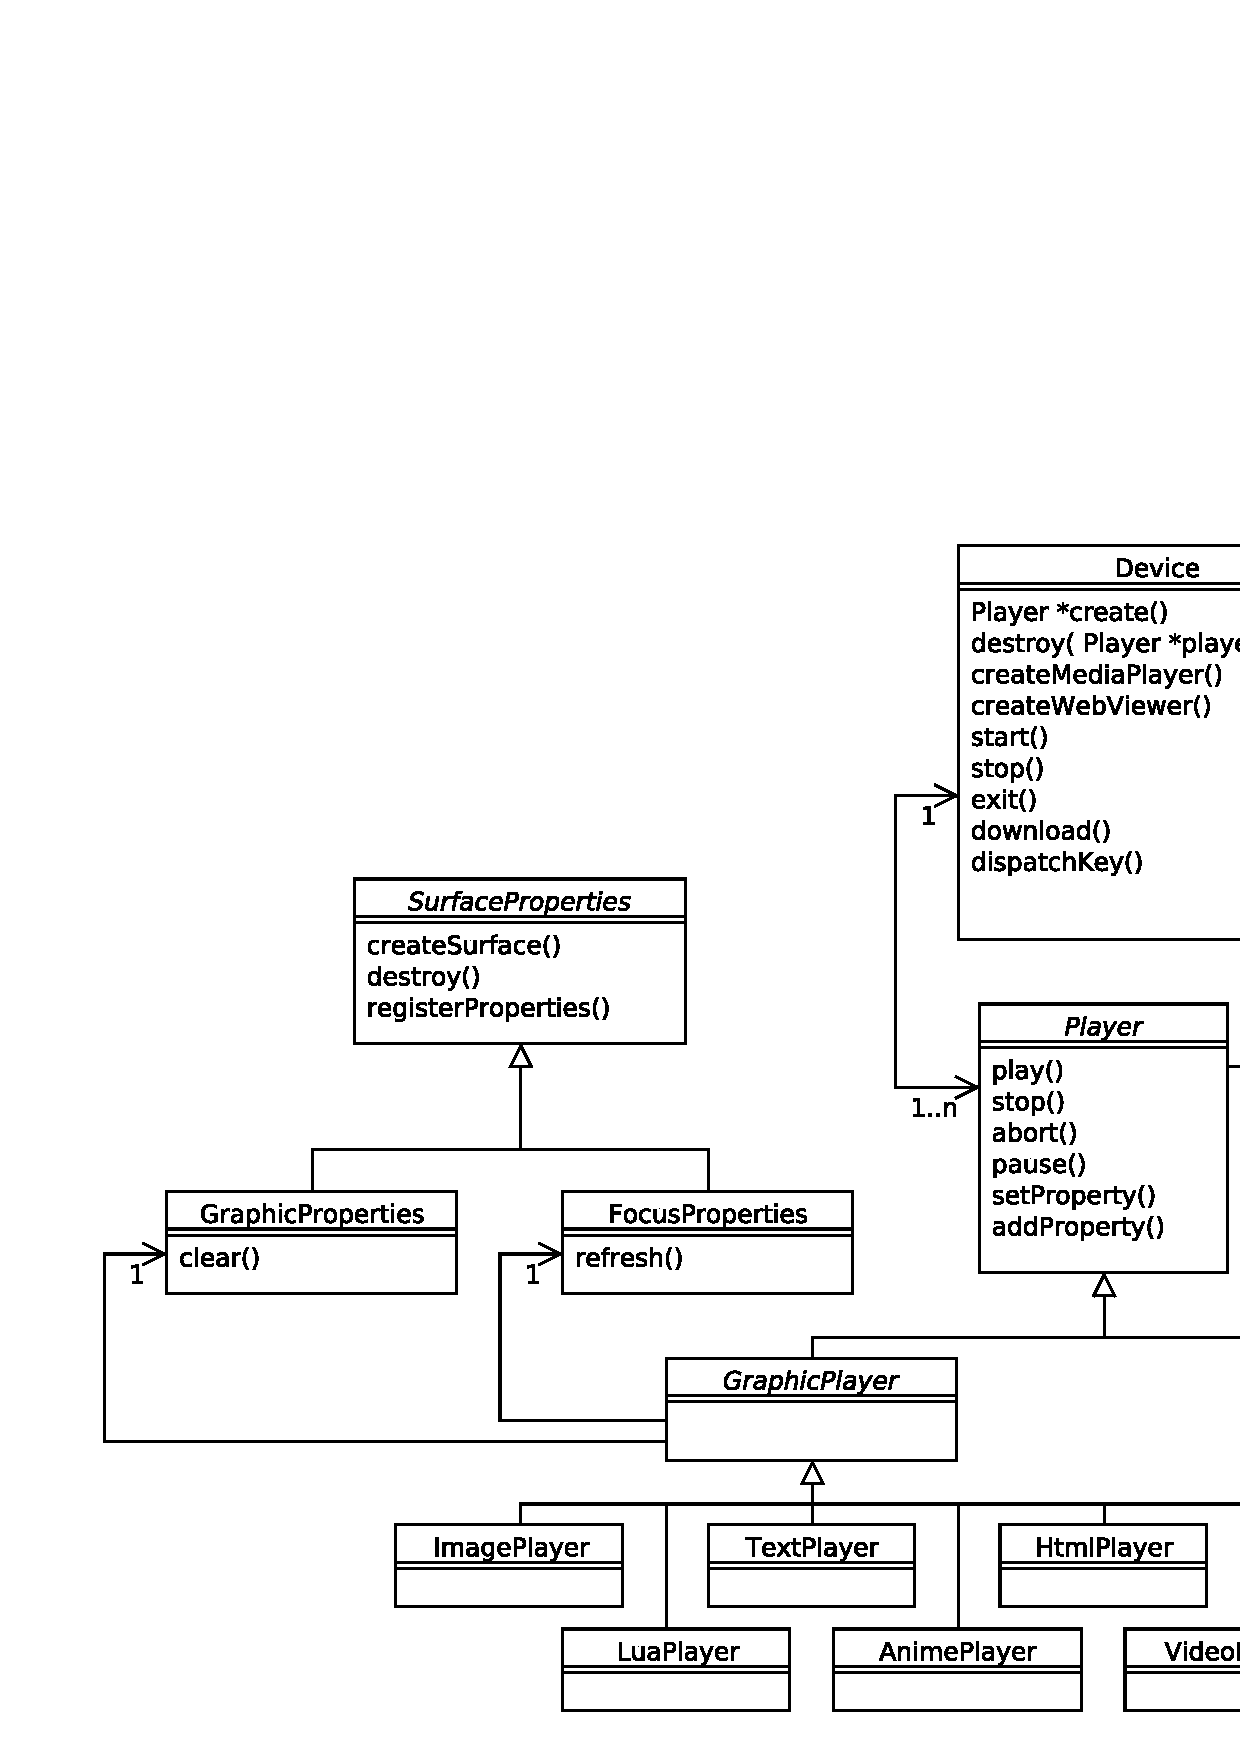
\includegraphics[scale=0.5]{resources/uml-dtv-gingaplayer.jpg}
	\caption{Diagrama de las principales clases de la librería \emph{gingaplayer}.}
\end{figure}

\FloatBarrier
